\documentclass[border=3pt]{standalone}

% Drawing
\usepackage{tikz}
\usetikzlibrary{angles, quotes, intersections}

% Notation
\usepackage{physics}
\usepackage{bm}
\usepackage{xcolor}

\newcommand{\PlaceCoordinates}{%
    \coordinate (P) at (5,0);
    \coordinate (O) at (0,0);
    \coordinate (Q) at (3,2);
    \coordinate (Qp) at (3,3.5);
    \coordinate (R) at (2.2,2.8);
}

\begin{document}

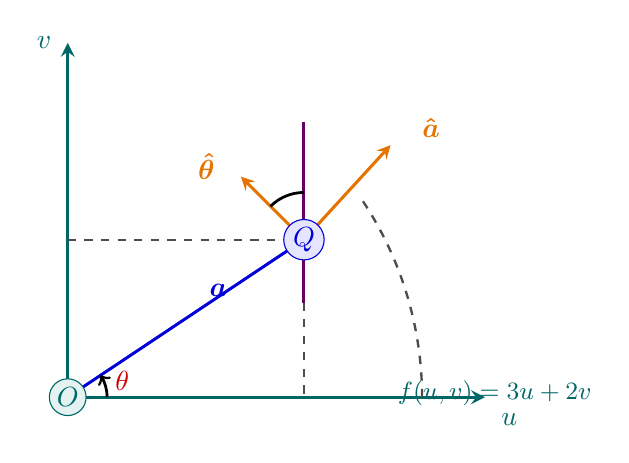
\begin{tikzpicture}
    % Coordinates
    \PlaceCoordinates

    % Axes
    \draw[line width=1.2pt, teal!80!black, -stealth] (-1ex,0) -- (5.3,0) node[below right=2pt] {\textcolor{teal!80!black}{$u$}};
    \draw[line width=1.2pt, teal!80!black, -stealth] (0,-1ex) -- (0,4.5) node[left=2pt] {\textcolor{teal!80!black}{$v$}};

    % Vectors
    \draw[line width=1.1pt, blue!85!black] (0,0) -- (3,2) node[pos=0.52, above right=3pt] {\textcolor{blue!85!black}{$\bm{a}$}};
    \draw[line width=1.1pt, orange!90!black, -stealth] (3,2) -- (4.1,3.2) node[pos=1.18, right=2pt] {\textcolor{orange!90!black}{$\vu*{a}$}};
    \draw[line width=1.1pt, orange!90!black, -stealth] (3,2) -- (2.2,2.8) node[pos=1.16, left=2pt] {\textcolor{orange!90!black}{$\vu*{\theta}$}};

    % Helper Lines
    \draw[dashed, line width=0.85pt, gray!60!black] (0,2) -- (3,2) -- (3,0);
    \draw[line width=1.1pt, violet!80!black] (3,3.5) -- (3,1.2);
    \draw[dashed, line width=0.85pt, gray!60!black] (4.5,0) arc (0:33.7:4.5);

    % Angles
    \pic[draw, ->, line width=1pt, "$\theta$", angle eccentricity=1.45, text=red!80!black] {angle = P--O--Q};
    \pic[draw, line width=1pt, angle radius=6mm, angle eccentricity=1.45, text=violet!80!black] {angle = Qp--Q--R};

    % Labels (Nodes)
    \node[fill=teal!10!white, draw=teal!80!black, circle, inner sep=1pt] at (O) {\textcolor{teal!80!black}{$O$}};
    \node[fill=blue!10!white, draw=blue!85!black, circle, inner sep=1pt] at (Q) {\textcolor{blue!85!black}{$Q$}};

    % Equation
    \node[below right=2pt, font=\small\bfseries, text=teal!80!black] at (4,0.4) {$f(u,v)=3u+2v$};

\end{tikzpicture}

\end{document}
